\documentclass[10pt]{article}

\usepackage{../../course-specific/course-head}

\newcommand{\blattnr}{0}

\begin{document}
    \makecover

    \begin{aufgabe}[0]
        Zeigen oder widerlegen Sie:
    \end{aufgabe}

    \begin{loesung}
        \begin{enumerate}
            \item \textsl{$3^n = \O(2^n)$}

            \begin{gegenbeweis}
                Es sei $A := 3^n = \O(2^n)$, sodass $A(n) \iff \exists c > 0 \; \exists n_0 > 0 \; \forall n > n_0 : 0 \leq 3^n \leq c \cdot 2^n$.
                Wir betrachten das Grenzwertverhalten von $\left[\frac{2^n}{3^n}\right]$ für $n \to \infty$ und erwarten nach $A(n)$, dass $\limsup_{n \to \infty} \frac{2^n}{3^n} \in (0, \infty]$.
                \[
                    \limsup_{n \to \infty} \frac{2^n}{3^n} = \limsup_{n \to \infty} \left(\frac{2}{3}\right)^n = 0
                \]
                $\limsup_{n \to \infty} \frac{2^n}{3^n} = 0$ und $A(n)$ gilt nicht.
            \end{gegenbeweis}

            \item \textsl{Es sei $G = (V, E)$ ein ungerichteter Graph mit $\abs{V} \geq 1$.
            Es gilt $\sum_{v \in V} \deg(v) = 2 \abs{E}$.}

            \begin{beweis}
                Diese Aussage ($A(G)$) zeigen wir auch mittels vollständiger Induktion.
                \IB Wir betrachten $G$ so, dass $\abs{V} = 1$.
                Dann ist $\abs{E} = 0$ und es gilt
                \[
                    \sum_{v \in V} \deg(v) = 0 = 2 \cdot 0 = 2 \abs{E}.
                \]

                \IA Für einen beliebigen (ungerichteten) Graphen $G$ gilt $A(G)$.

                \IS[1] Wir betrachten zunächst den Fall, in dem wir $G$ um einen Knoten zu $G' := (V', E)$ mit $\abs{V'} = \abs{V} + 1$ erweitern.
                Dann ist $\sum_{v \in V} \deg(v) = \sum_{v' \in V'} \deg(v')$.
                An der Aussage verändert sich also nichts und unter \textsf{(I. A.)} gilt auch $A(G')$.

                \IS[2] Im nächsten Schritt wollen wir den Graphen $G$ um eine Kante zu $G' = (V', E')$ mit $\abs{E'} = \abs{E} + 1$ erweitern.
                Eine Kante lässt sich genau dann zwischen zwei Knoten $v_i, v_j$ platzieren, falls zwischen $v_i$ und $v_j$ noch keine Kante existiert.
                Es sei dazu $\mathbf{A} = [a_{kl}]$ die Adjazenzmatrix von $G$, wobei
                \[
                    a_{kl} :=
                    \begin{cases}
                        1, & \text{falls } \{v_k, v_l\} \in E\\
                        0 & \text{sonst.}
                    \end{cases}
                \]
                Daraus ergibt sich die Menge der Tupel von Knoten, zwischen denen sich Kanten platzieren lassen, wie folgt:
                \[
                    E_n = \{\{v_i, v_j\} \mid \forall i,j \in \{1,2, \cdots, \abs{V}\}(\mathbf{A}_{ij} = 0)\}.
                \]
                Fügen wir dann eine Kante zwischen zwei beliebigen Knoten $v_i, v_j$ (wobei $\{v_i, v_j\} \in E_n$) ein, so erhöht sich der Grad beider Knoten um $1$.
                Daraus ergibt sich
                \[
                    \sum_{v' \in V'} \deg(v') = \sum_{v \in V} \deg(v) + 2 \stackrel{\textsf{(I.A.)}}{=} 2 (\abs{E} + 1) = 2 \abs{E'}.
                \]

                Aus \textsf{(I.S. 1)} und \textsf{(I.S. 2)} lässt sich jeder beliebige Graph $G = (E, V)$ (mit beliebig vielen Zusammenhangskomponenten) erzeugen und wir haben gezeigt, dass $\sum_{v \in V} \deg(v) = 2 \abs{E}$ gilt.
            \end{beweis}

            \item In jedem (binären) Heap $H$ gilt für die Anzahl Blätter $b(H)$ und die Anzahl Nicht-Blätter $n(H)$:
            \[
                n(H) \leq b(H) \leq n(H) + 1.
            \]

            \begin{beweis}
                Es sei also $A$ die Aussageform und $H$ ein beliebiger Heap, sodass
                \[
                    A(H) := [n(H) \leq b(H) \leq n(H) + 1].
                \]
                Ferner sei $\abs{H}$ die Anzahl der Knoten des Heaps und wir betrachten zunächst den Basisfall, in dem $\abs{H} = 1$.

                \IB $\abs{H}$ ist $1$ und der Knoten ist gleichzeitig auch ein Blatt.
                Dann ist $n(H) = 0$, $b(H) = 1$ und es gilt $n(H) \leq b(H) \leq n(H) + 1$ mit
                \[
                    0 \leq 1 \leq 1.
                \]
                Dann können wir die Induktionsannahme wie folgt formulieren.
                \IA Für einen beliebigen Heap $H$ gilt $n(H) \leq b(H) \leq n(H) + 1$.
                Unter dieser Annahme können wir dann 2 atomare Fälle, also Teilbäume betrachten, aus denen sich ein beliebig gro{\ss}er Heap konstruieren lässt.
                \IS[1] Unter der Annahme, dass für einen beliebigen Heap $A(H)$ gilt, fügen wir einen Knoten $v_2$ an einen Knoten $v_1$ (\autoref{fig:figure1}).
                Es kommt also kein neues Blatt hinzu.
                Dann ist $\abs{H'} := \abs{H} + 1$, $n(H') := n(H) + 1$, $b(H') = b(H)$ und daraus folgt für $A(H')$
                \[
                    [n(H') \leq b(H') \leq n(H') + 1] := [n(H) + 1 \leq b(H) \leq (n(H) + 1) + 1].
                \]
                Insbesondere muss nun noch gezeigt werden, dass $n(H) < b(H)$, sodass wir zeigen können, dass $A(H')$ gilt.
                Wir wissen, dass ein Heap linksvollständig ist.
                Damit ist auch gegeben, dass ein Hinzufügen nach~\autoref{fig:figure1} nur möglich ist gdw. sowohl alle Ebenen bis zur Höhe des Knotens $v_1$ vollständig sind, als auch alle linken Geschwisterknoten mindestens und genau 2 Nachfolger haben.
                Und ein Teilbaum ist vollständig gdw. er zwei Nachfolger hat.
                Das ist die maximale Anzahl an Nachfolgern eines Knotens in einem binären Baum.
                Der Teilbaum enthält dann lokal zwei Blätter und ein Nicht-Blatt.
                Dann ist $b(H) = n(H) + 1$ und daraus folgt wie gewünscht $n(H) < b(H)$.

                \IS[2] Wir betrachten dann den Fall, in dem ein beliebiger Knoten $v_1$ in einem Heap genau einen Nachfolger hat.
                Um die Linksvollständigkeit nicht zu verletzen, erfolgt das Hinzufügen eines Knotens $v_3$ dann zwangsläufig als zweiter nachfolgende Knoten von $v_1$~\autoref{fig:figure2} und $v_3$ ist dann ein Blatt.
                Ein Hinzufügen nach diesem Schema kann also nur auf ein Hinzufügen nach~\autoref{fig:figure1} folgen.
                Betrachten wir also wieder ein $H$ vor \textsf{(I.S. 1)} und zeigen $A(H'')$ mittels der Gültigkeit von $A(H')$.
                \[
                    [n(H'') \leq b(H'') \leq n(H'') + 1] := [n(H') \leq b(H') + 1 \leq n(H') + 1],
                \]
                wobei $b(H) = n(H) + 1 \stackrel{\textsf{(I.S. 1)}}{\implies} b(H') = n(H') \implies n(H') < b(H') + 1 = n(H') + 1$ und für jedes beliebige Heap $H$ gilt $n(H) \leq b(H) \leq n(H) + 1$.
            \end{beweis}
            \begin{figure}[h]
                \caption{Induktionsschritte}
                \centering
                \begin{subfigure}{.3\textwidth}
                    \caption{{\sf(I.S. 1)}}
                    \\[1pt]
                    \centering
                    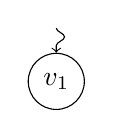
\begin{tikzpicture}[nodes={draw, circle}, ->, local bounding box=bb,baseline=(bb.center),scale=0.9,node distance= 2cm]
                        \node (v1) {$v_1$};
                        \draw[decorate,decoration={snake,amplitude=3pt,post length=1pt}]  (0,0.75) -- (v1);
                    \end{tikzpicture} \Rightarrow
                    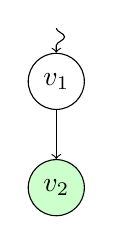
\begin{tikzpicture}[nodes={draw, circle}, ->, local bounding box=bb,baseline=(bb.center),scale=0.9]
                        \node (v1) at (0, 0) {$v_1$};
                        \node[fill=green!20] (v2) at (0, -1.5) {$v_2$};
                        \draw[->] (v1) -- (v2);
                        \draw[decorate,decoration={snake,amplitude=3pt,post length=1pt}]  (0,0.75) -- (v1);
                    \end{tikzpicture}\label{fig:figure1}
                \end{subfigure}
                \begin{subfigure}{.3\textwidth}
                    \caption{{\sf(I.S. 2)}}
                    \\[1pt]
                    \centering
                    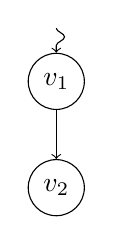
\begin{tikzpicture}[nodes={draw, circle}, ->, local bounding box=bb,baseline=(bb.center),scale=0.9]
                        \node (v1) at (0, 0) {$v_1$};
                        \node (v2) at (0, -1.5) {$v_2$};
                        \draw[->] (v1) -- (v2);
                        \draw[decorate,decoration={snake,amplitude=3pt,post length=1pt}]  (0,0.75) -- (v1);
                    \end{tikzpicture} \Rightarrow
                    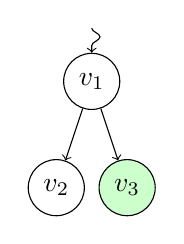
\begin{tikzpicture}[nodes={draw, circle}, ->, local bounding box=bb,baseline=(bb.center),scale=0.9]
                        \node (v1) at (0, 0) {$v_1$};
                        \node (v2) at (-0.5, -1.5) {$v_2$};
                        \node[fill=green!20] (v3) at (0.5, -1.5) {$v_3$};
                        \draw[->] (v1) -- (v2);
                        \draw[->] (v1) -- (v3);
                        \draw[decorate,decoration={snake,amplitude=3pt,post length=1pt}]  (0,0.75) -- (v1);
                    \end{tikzpicture}\label{fig:figure2}
                \end{subfigure}
            \end{figure}
        \end{enumerate}
    \end{loesung}
\end{document}